\newpage


\section{Profile Guided Optimizations}



\subsection{Improved Basic Block Reordering}

Improved Basic Block Reordering \cite{newell2020improved} is published by Andy Newell and Sergey Pupyrev
from Facebook. 


Given a directed control flow graph comprising of basic blocks and frequencies of jumps between the blocks, find an ordering
of the blocks such that the number of fall-through jumps
is maximized. This is the maximum directed TRAVELING
SALESMAN PROBLEM (TSP). Solving TSP alone is not sufficient for constructing a good ordering of basic blocks. It is easy to find
examples of control flow graphs with multiple different
orderings that are all optimal with respect to the TSP objective. Consider for example a control flow graph in Figure \ref{fig:p54}
in which the maximum number of fall-through branches is
achieved with two orderings that utilize a different number
of I-cache lines in a typical execution. For these cases, an
algorithm needs to take into consideration non-fall-through
branches to choose the best ordering. However, maximizing the number of fall-through jumps is not always preferred
from the performance point of view. Consider a control
flow graph with seven basic blocks in Figure \ref{fig:p55}. It is not hard
to verify that the ordering with the maximum number of
fall-through branches is one containing two concatenated
chains, B0$\rightarrow$B1$\rightarrow$B3$\rightarrow$B4 and B5$\rightarrow$B6$\rightarrow$B2 (upper-right in
Figure \ref{fig:p55}). Observe that for this placement, the hot part of
the function occupies three 64-byte cache lines. Arguably a
better ordering is the lower-right in Figure \ref{fig:p55}, which uses only
two cache lines for the five hot blocks, B0, B1, B2, B3, B4, at
the cost of breaking the lightly weighted branch B6$\rightarrow$B2.



\begin{figure}[H]
    \centering
     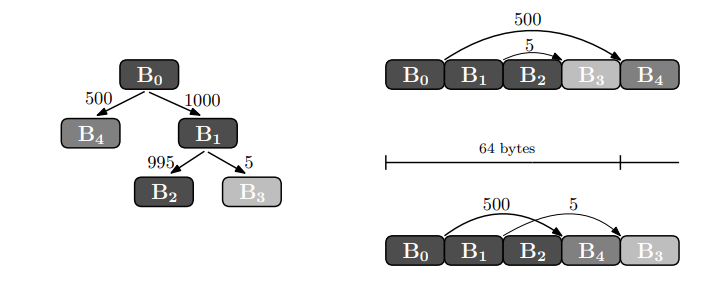
\includegraphics[width=0.5\textwidth]{p54.png}
         \caption{ Two orderings of basic blocks with the same TSP score (1995)
         resulting in different I-cache utilization. All blocks have the same size of
         16 bytes and colored according to their hotness in the profile.}
         \label{fig:p54}
\end{figure}


\begin{figure}[H]
    \centering
     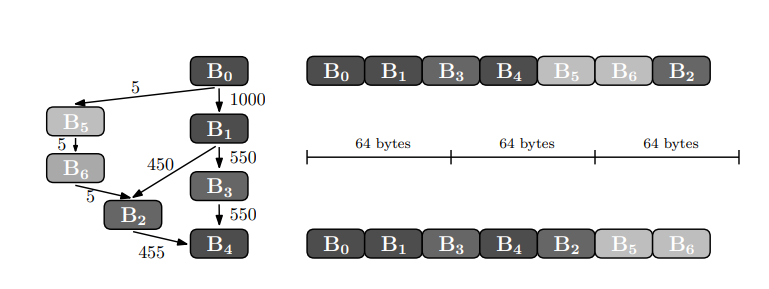
\includegraphics[width=0.5\textwidth]{p55.png}
         \caption{A control flow graph with jump frequencies (left) and two possible
         orderings of basic blocks (right). All blocks have the same size (in bytes)
         and colored according to their hotness in the profile. An optimal TSPbased layout (upper right) utilizes three cache lines for the hot code,
         while an arguably better layout (lower right) can be built with a new
         EXTTSP model.}
         \label{fig:p55}
\end{figure}


\subsubsection{Contribution}

The contributions of the paper are the following.

\begin{itemize}
\item  Identify an opportunity for improvement over the
classical approach for basic block reordering, initiated
by Pettis and Hansen \cite{pettis1990profile}. Then they extend the model and
suggest a new optimization problem with the objective
closely related to the performance of a binary.

\item Develop a new practical algorithm for basic
block reordering. The algorithm relies on a greedy
technique for solving the optimization problem.

\item Propose a Mixed Integer Programming formulation
for the aforementioned optimization problem, which is
capable of finding optimal solutions on small functions
\end{itemize}

\subsubsection{New ideas}

In their study, they consider the following features.

\begin{itemize}
\item The length of a jump impacts the performance of instruction caches. Longer jumps are more likely to result
in a cache miss than shorter ones. In particular, a jump
with the length shorter than 64 bytes has a chance to
remain within the same cache line.

\item The direction of a branch plays a role for branch predicting. A branch s$\rightarrow$t is called forward if s $<$ t, that is,
block s precedes block t in the ordering; otherwise, the
branch is called backward.

\item The branches can be classified into unconditional (if the
out-degree is one) and conditional (if the out-degree is
two). A special kind of branches is between consecutive
blocks in the ordering that are called fall-through; in this
case, a jump instruction is not needed.

\item They introduce a new score that estimates the quality
of a basic block ordering taking into account the branch
characteristics. In the most generic form, the new function,
called EXTENDED TSP (EXTTSP), is expressed as follows:

$$\operatorname{ExtTSP}=\sum_{(s, t)} w(s, t) \times K_{s, t} \times h_{s, t}(\operatorname{len}(s, t))$$


where the sum is taken over all branches in the control
flow graph. Here $w(s, t)$ is the frequency of branch s$\rightarrow$t and
$0 \leq K_{s,t} \leq 1$ is a weight coefficient modeling the relative
importance of the branch for optimization. We distinguish
six types of branches arising in code: conditional and unconditional versions of fall-through, forward, and backward
branches. Thus, we introduce six coefficients for EXTTSP.
The lengths of the jumps are accounted in the last term of the
expression, which increases the importance of short jumps.
A non-negative function $h_{s,t}(len(s, t))$ is defined by value
of 1 for zero-length jumps, value of 0 for jumps exceeding a
prescribed length, and it monotonically decreases between
the two values. To be consistent with the objective of TSP,
the EXTTSP score needs to be maximized for the best performance. Notice that EXTTSP is a generalization of TSP, as the
latter can be modeled by setting $K_{s,t} = 1, h(len(s, t)) = 1$
for fall-through branches and $K_{s,t} = 0$ otherwise.


\end{itemize}


They use machine learning methods to find parameters for EXTTSP
that have the highest correlation with the performance of
a binary in the experiment. 



$$
\operatorname{ExtTSP}=\sum_{(s, t)} w(s, t) \times \begin{cases}1 & \text { if } \operatorname{len}(s, t)=0, \\ 0.1 \cdot\left(1-\frac{\operatorname{len}(s, t)}{1024}\right) & \text { if } 0<\operatorname{len}(s, t) \leq 1024 \\ & \text { and } s<t, \\ 0.1 \cdot\left(1-\frac{\operatorname{len}(s, t)}{640}\right) & \text { if } 0<\operatorname{len}(s, t) \leq 640 \\ & \text { and } t<s, \\ 0 & \text { otherwise. }\end{cases}
$$

.
Intuitively, EXTTSP resembles the traditional TSP
model, as the number of fall-through branches is the dominant factor. The main difference is that EXTTSP rewards
longer jumps. The impact of such jumps is significantly
lower and it linearly decreases with the length of a jump.
Next we summarize our high-level observations regarding
the new score function.

\subsubsection{Algorithm}

\begin{algorithm}[H]
    \caption{Basic Block Reordering}\label{alg:Basic Block Reordering}
    \begin{algorithmic}
    \State{\textbf{Input: }  control flow graph $G = (V, E, w)$, the entry point $v^\star \in V$ }
    \State{\textbf{Output: } ordering of basic blocks ($v^\star = B_1, B_2,\dots,B_{|v|}$)}
    \Function{ReorderBasicBlocks}{}
    \For{$v \in V$}
    \State{$Chains \gets Chains \cup (v)$}
    \EndFor
    \While{ $|Chains| > 1$} \Comment{chain merging}
    \For{$c_i,c_j \in Chains$}
    \State{$gain[c_i,c_j] \gets$  ComputeMergeGain($c_i, c_j$ )}
    \EndFor
    \State{$\operatorname{src}, d s t \leftarrow \underset{i, j}{\arg \max } \operatorname{gain}\left[c_i, c_j\right]$}  \Comment{find best pair of chains}
    \State {$Chains \gets Chains \cup Merge(src, dst) \backslash \{src, dst\};$} \Comment{merge the pair and update chains}
    \EndWhile{\\}
    \Return{ordering given by the remaining chain;}
    \EndFunction


    \Function{ComputeMergeGain}{src, dst}
    \For{$i=1$ \textbf{to} blocks(src)} \Comment{try all ways to split chain src}
    \State{$s_1 \gets src[1:i]$} \Comment{break the chain at index i}
    \State{$s_2 \gets src[i+1:blocks(src)]$}
    \State{score $_i \leftarrow \max \left\{\begin{array}{l}\operatorname{ExtTSP}\left(s_1, s_2, d s t\right) \text { if } v^* \notin d s t \\ \operatorname{ExtTSP}\left(s_1, d s t, s_2\right) \text { if } v^* \notin d s t \\ \operatorname{ExtTSP}\left(s_2, s_1, d s t\right) \text { if } v^* \notin s_1, d s t \\ \operatorname{ExtTSP}\left(s_2, d s t, s_1\right) \text { if } v^* \notin s_1, d s t \\ \operatorname{ExtTSP}\left(d s t, s_1, s_2\right) \text { if } v^* \notin s r c \\ \operatorname{ExtTSP}\left(d s t, s_2, s_1\right) \text { if } v^* \notin s r c\end{array}\right.$} \Comment{try all valid ways to concatenate}
    \EndFor{\\}
    \Return{$\max _i$ score $_i-\operatorname{ExtTSP}(s r c)-\operatorname{ExtTSP}(d s t)$} \Comment{ the gain of merging chains src and dst}
    \EndFunction
    \end{algorithmic}
    \end{algorithm}








    